\documentclass[11pt]{article}
\usepackage[margin=0.9in]{geometry}
\usepackage{amsmath,amssymb,amsthm,mathtools}
\usepackage{graphicx}
\usepackage{microtype}
\usepackage[hidelinks]{hyperref}

\newtheorem{theorem}{Theorem}
\newtheorem{lemma}{Lemma}
\newtheorem{corollary}{Corollary}
\newcommand{\F}{\mathbb F}
\newcommand{\C}{\mathbb C}
\newcommand{\R}{\mathbb R}

\title{Sharp Norms for Involutory Dilations\\
\large Candidate full answers to Questions 3.2 and 3.4 of arXiv:2602.19599}
\author{Autonomous proof candidate for human review}
\date{11 August 2026}

\begin{document}
\maketitle

\begin{center}
\fbox{\parbox{0.91\textwidth}{\textbf{Status.}
Candidate full resolution, likely valid.  The involution already displayed
in Proposition 3.3 of the source has the exact operator norm
\(\|A\|+\sqrt{1+\|A\|^2}\).  This gives a real-preserving dilation in
dimension \(2n\), improves the constant \(3\) sharply to \(1+\sqrt2\), and,
apart from the elementary real one-dimensional exception described below,
attains the smallest possible universal norm.}}
\end{center}

\section{The questions and the answer}

For a matrix \(A\in M_n(\F)\), where \(\F=\R\) or \(\C\), the source
introduces the involution
\begin{equation}\label{eq:SA}
 S_A=\begin{pmatrix}A&I+A\\ I-A&-A\end{pmatrix}\in M_{2n}(\F)
\end{equation}
and proves \(\|S_A\|\le 1+2\|A\|\).  Question 3.2 asks whether a real
contraction has a real involutory dilation with the sharp norm
\(1+\sqrt2\).  Question 3.4 asks for the sharp replacement of \(3\) in the
bound for \(S_A\), and whether that replacement is also the optimal norm
for arbitrary involutory dilations in dimension \(2n\).

\begin{figure}[ht]
 \centering
 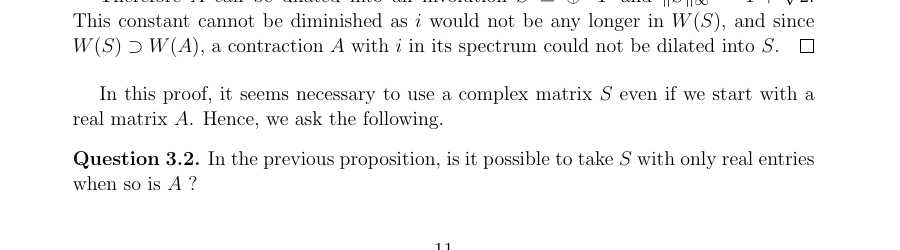
\includegraphics[width=0.96\textwidth]{figures/question_3_2.png}
 \vspace{4pt}
 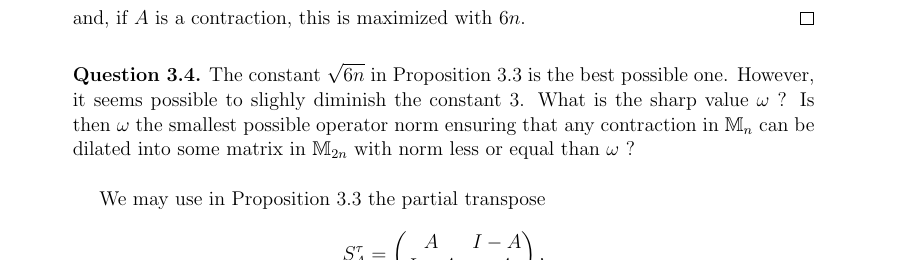
\includegraphics[width=0.96\textwidth]{figures/question_3_4.png}
 \caption{Questions 3.2 and 3.4 in the source, PDF pages 11 and 12.}
\end{figure}

\begin{theorem}\label{thm:main}
For every \(A\in M_n(\F)\),
\begin{equation}\label{eq:normformula}
 \boxed{\ \|S_A\|=\|A\|+\sqrt{1+\|A\|^2}\ }.
\end{equation}
Consequently:
\begin{enumerate}
\item every contraction has an involutory dilation in \(M_{2n}(\F)\) of
      norm at most \(1+\sqrt2\), with no change of scalar field;
\item the sharp constant replacing \(3\) for the family \(S_A\) is
      \(\omega=1+\sqrt2\);
\item the least universal norm for involutory dilations in \(M_{2n}(\C)\)
      is \(1+\sqrt2\).  The same is true in \(M_{2n}(\R)\) when \(n\ge2\).
\end{enumerate}
For real \(n=1\) only, the least universal norm in the last assertion is
\(1\), although the sharp uniform bound for the specific matrices \(S_A\)
remains \(1+\sqrt2\).
\end{theorem}

Thus Question 3.2 is answered affirmatively in a stronger dimension
\(2n\) form.  If the statement is read as requiring exactly dimension
\(4n\) and norm exactly \(1+\sqrt2\), both can also be retained; see
Corollary~\ref{cor:real4n}.

\section{A two-line unitary reduction}

Set
\[
 H=\frac1{\sqrt2}\begin{pmatrix}I&I\\I&-I\end{pmatrix}.
\]
This matrix is orthogonal (and unitary), self-adjoint, and a direct block
multiplication gives
\begin{equation}\label{eq:reduction}
 HS_AH=Q_A:=\begin{pmatrix}I&0\\2A&-I\end{pmatrix}.
\end{equation}
In particular, \(S_A^2=I\) is also transparent from this form.

\begin{lemma}\label{lem:blocknorm}
For every operator \(A\) on a finite-dimensional real or complex Hilbert
space, if \(a=\|A\|\), then
\[
 \left\|\begin{pmatrix}I&0\\2A&-I\end{pmatrix}\right\|
 =a+\sqrt{1+a^2}.
\]
\end{lemma}

\begin{proof}
For vectors \(x,y\), put \(p=\|x\|\) and \(q=\|y\|\).  The triangle
inequality gives
\begin{align*}
 \|Q_A(x,y)\|^2
 &=\|x\|^2+\|2Ax-y\|^2\\
 &\le p^2+(2ap+q)^2
 =\begin{pmatrix}p&q\end{pmatrix}
   \begin{pmatrix}1+4a^2&2a\\2a&1\end{pmatrix}
   \begin{pmatrix}p\\q\end{pmatrix}.
\end{align*}
The largest eigenvalue of the displayed scalar matrix is
\[
 1+2a^2+2a\sqrt{1+a^2}
 =\bigl(a+\sqrt{1+a^2}\bigr)^2.
\]
This proves the upper bound.  If \(a>0\), choose a unit vector \(x\) with
\(\|Ax\|=a\), put \(z=Ax/a\), and restrict to pairs \((rx,-tz)\) with
\(r,t\ge0\).  On this two-dimensional set the preceding quadratic form is
attained exactly, so its maximal Rayleigh quotient gives the matching lower
bound.  If \(a=0\), then \(Q_A=\operatorname{diag}(I,-I)\), and the formula
again holds.
\end{proof}

Because \(H\) is unitary, equations \eqref{eq:reduction} and
Lemma~\ref{lem:blocknorm} prove \eqref{eq:normformula}.  Since the upper-left
corner of \(S_A\) is \(A\), it is an involutory dilation of \(A\).  It has
the same real or complex entries as \(A\), proving the upper-bound and
real-preservation assertions.  The function
\(a\mapsto a+\sqrt{1+a^2}\) is increasing, and equality at \(a=1\) shows
that the uniform constant for \(S_A\) is sharply \(1+\sqrt2\).

\section{Optimality among all involutory dilations}

We include the short lower-bound argument to distinguish the norm of the
specific formula \(S_A\) from the optimum over all possible dilations.
If \(A=V^*SV\) is a compression, then \(W(A)\subseteq W(S)\).  For an
involution of norm \(s\), Corollary 2.3(d) of the source gives the numerical
range as an ellipse whose vertical semiaxis is
\begin{equation}\label{eq:vertical}
 \frac{s-s^{-1}}2.
\end{equation}
Over \(\C\), take the contraction \(A=iI_n\).  Then \(i\in W(A)\), so
\eqref{eq:vertical} is at least \(1\).  Hence
\(s-s^{-1}\ge2\), equivalently \(s\ge1+\sqrt2\).  Formula
\eqref{eq:SA} supplies the matching \(2n\)-dimensional upper bound.

For real \(n\ge2\), take
\[
 A=\begin{pmatrix}0&-1\\1&0\end{pmatrix}\oplus0_{n-2}.
\]
Complexifying any proposed real involutory dilation preserves its norm and
compression relation, while the complexification of \(A\) has eigenvalue
\(i\).  The same lower bound therefore applies.  When \(n=1\), however,
each scalar contraction \(a\in[-1,1]\) has the orthogonal involutory
dilation
\[
 R_a=\begin{pmatrix}a&\sqrt{1-a^2}\\
          \sqrt{1-a^2}&-a\end{pmatrix},
 \qquad R_a^2=I,\quad \|R_a\|=1.
\]
No involution can have norm below its spectral radius \(1\), proving the
stated exceptional value.

\begin{corollary}\label{cor:real4n}
If \(A\in M_n(\R)\) is a contraction, there is a real involution
\(\widetilde S\in M_{4n}(\R)\) dilating \(A\) with
\(\|\widetilde S\|=1+\sqrt2\).
\end{corollary}

\begin{proof}
Let
\[
 T=\begin{pmatrix}0&1+\sqrt2\\\sqrt2-1&0\end{pmatrix}.
\]
Then \(T^2=I\) and \(\|T\|=1+\sqrt2\).  The real block direct sum
\(\widetilde S=S_A\oplus T^{\oplus n}\) has size \(4n\), still contains
\(A\) as its leading compression, and has the required norm.
\end{proof}

\section{Verification, novelty, and scope}

The accompanying script \texttt{code/verify\_involutory\_dilation.py}
checks \(S_A^2=I\) and the Hadamard identity exactly over random rational
matrices, then compares the singular-value norm with
\eqref{eq:normformula} for real and complex matrices over several sizes and
scales.  It also verifies the exact scalar characteristic polynomial used
in Lemma~\ref{lem:blocknorm}.

A bounded search on 11 August 2026 found only version 1 of the source and no
later arXiv paper stating \eqref{eq:normformula} or answering Questions 3.2
and 3.4.  The construction \eqref{eq:SA}, the numerical-range ellipse, and
the optimal lower-bound example are all already present in the source; the
new step claimed here is the fixed Hadamard reduction and exact norm
calculation, together with its consequences.  Priority is not asserted.

\end{document}
